\documentclass[../thesis.tex]{subfiles}
\begin{document}

\chapter{Theory}
\label{chp:theory}

Within this chapter the theory and procedures needed to solve a CFD case are shown. At first a broad overview is given and the generic equations are laid out. That is then followed by the explanation of the solution algorithm that is used in this work.

Building a theoretical model describing the evolution of a reaction's species in time and space equations that are dependent of the special coordinates and time are needed. These equations should describe the flow field and species distribution in addition to other fluid flow related quantities. These equations have the characteristic of forming a partial differential equation (PDE) system for which no analytical solution can be computed. Solving these equations numerically has lead to the development of special approaches and solution techniques. All these methods are classified under the field of Computational Fluid Dynamics or CFD in short. The basic principles of this field are explained in \autoref{sec: CFD}. 
 
\section{Computational Fluid Dynamics}
\label{sec: CFD}

Computational fluid dynamics is the computer based solving of problems regarding fluid flow, heat transfer, chemical reactions or other phenomena. The concept is used in a large variety of applications within the fields of engineering and science for at least the last 60 years \cite{versteeg2007introduction}. Within \autoref{fig:cdf_procedure} the general procedure of solving a CFD case is shown.
\begin{figure}[htbp]
	\centering
	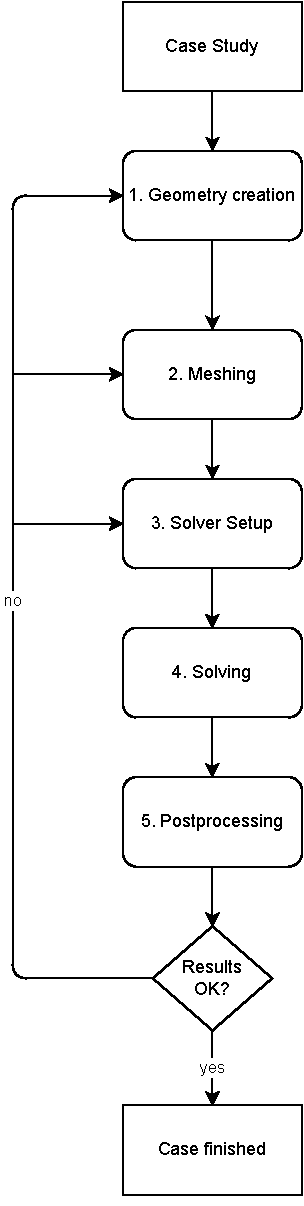
\includegraphics[height=\textheight]{CFD_general}
	\caption{CFD Case Procedure}
	\label{fig:cdf_procedure}
\end{figure}

The first step is to model the domains geometry. In case of \texttt{ANSYS FLUENT} this step can either be done within the CFD software itself or an external CAD program. After the geometry is created or imported form an external source a mesh needs to be created. This mesh is the basis for the solver to solve the case and an important step. The way the mesh is set up has a significant influence on the model's results and the computational resources needed. The finer the mesh the more computational power is needed for computing the solution. By lowering the grid's element size the resources needed or simulation time increases exponentially.

When meshing is finished the next step according to \autoref{fig:cdf_procedure} is the solver setup. Setting up the governing equations, simulation time and boundary conditions are tasks performed in this step. The setup is described in greater detail within \autoref{sec: setup}. After the solver is set up the case can be run by starting the solver. Depending on the resources needed or available this step needs some further configuration.

When the solving process has finished the obtained results can be inspected. If they contain errors some of the previous done steps might need to be revisited and adapted. Depending on the type of error the geometry or mesh need to be adapted as described in \autoref{fig:cdf_procedure}. Another common error is an incorrect solver setup. Correction here might involve changing the solver type or other related settings. How these steps are performed and what steps are taken to receive the final model are described in greater detail in \autoref{sec: mod_evol}.

All in all solving a CFD case is an iterative process that needs to be gone through multiple times until the results look as expected and can be trusted. That is why validation against experimental data is important to prove that the model shows valid behaviour and results. Further details on how these steps are performed while developing this specific model are given in \autoref{chp:model}.

\section{Governing Equations}
\label{sec:gov_eqn}
To obtain the results of interest the model needs to mainly solve a PDE system of three different equations. These equations are:
\begin{itemize}
	\item mass conservation equation
	\item energy equation
	\item reaction equation
\end{itemize}

\subsection{Mass Conservation}
To gain information about the velocity field the conservation equations for mass and momentum need to solved. For a 2D axisymmetric case as used here the equations look like this \cite{manual2009ansys}:

\begin{equation}
\label{eqn:ansys_conti}
\dfrac{\partial \rho}{\partial t} + \dfrac{\partial}{\partial x} (\rho u_x) + \dfrac{\partial }{\partial r} (\rho u_r)
+ \dfrac{\rho u_r}{r} = S_m
\end{equation}

This is the continuity equation for an in-compressible fluid where $r$ is the radial coordinate, $u_x$ is the axial velocity, $u_r$ is the radial velocity, $\rho$ is the density and $S_m$ is the source term. In addition to the shown continuity equation the radial and axial momentum equations need to be solved.

%\begin{equation}
%	\dfrac{\partial}{\partial t}(\rho u_x) + \dfrac{1}{r} \dfrac{\partial}{\partial x}(r \rho u_x^2)
%	+ \dfrac{1}{r} \dfrac{\partial}{\partial r}(r \rho u_r u_x) = 
%	- \dfrac{\partial p}{\partial x} + \dfrac{1}{r} \dfrac{\partial }{\partial x} \left[ 
%		r \mu \left( 2 \dfrac{\partial u_x}{\partial x} - \dfrac{2}{3}(\nabla \cdot \mathbf{u}) \right)
%	\right] + \dfrac{1}{r} \dfrac{\partial }{\partial r} \left[ 
%	r \mu \left( \dfrac{\partial u_x}{\partial r} - \dfrac{\partial u_r}{\partial x} \right)
%	\right]
%\end{equation}

\begin{gather}
	\dfrac{\partial}{\partial t}(\rho u_x) + \dfrac{1}{r} \dfrac{\partial}{\partial x}(r \rho u_x^2)
	+ \dfrac{1}{r} \dfrac{\partial}{\partial r}(r \rho u_r u_x) = 
	- \dfrac{\partial p}{\partial x} + \dfrac{1}{r} \dfrac{\partial }{\partial x} \left[ 
	r \mu \left( 2 \dfrac{\partial u_x}{\partial x} - \dfrac{2}{3}(\nabla \cdot \mathbf{u}) \right)
	\right] + \\ \nonumber
	\dfrac{1}{r} \dfrac{\partial }{\partial r} \left[ 
	r \mu \left( \dfrac{\partial u_x}{\partial r} - \dfrac{\partial u_r}{\partial x} \right)
	\right]	
\end{gather}

%\begin{equation}
%	\dfrac{\partial}{\partial t}(\rho u_r) + \dfrac{1}{x} \dfrac{\partial}{\partial r}(r \rho u_x u_r)
%	+ \dfrac{1}{r} \dfrac{\partial}{\partial x}(r \rho u_r^2) = 
%	- \dfrac{\partial p}{\partial r} + \dfrac{1}{r} \dfrac{\partial }{\partial x} \left[ 
%	r \mu \left( \dfrac{\partial u_r}{\partial x} - \dfrac{\partial u_x}{\partial r} \right)
%	\right]
%	+ \dfrac{1}{r} \dfrac{\partial }{\partial r} \left[ 
%	r \mu \left( 2 \dfrac{\partial u_r}{\partial r} - \dfrac{2}{3}(\nabla \cdot \mathbf{u}) \right)
%	\right] -
%	2 \mu \dfrac{u_r}{r^2}+ \dfrac{2}{3} \dfrac{\mu}{r}(\nabla \cdot \mathbf{u}) + \rho \dfrac{u_z^2}{r} + %F_r
%\end{equation}

\begin{gather}
	\dfrac{\partial}{\partial t}(\rho u_r) + \dfrac{1}{x} \dfrac{\partial}{\partial r}(r \rho u_x u_r)
	+ \dfrac{1}{r} \dfrac{\partial}{\partial x}(r \rho u_r^2) = 
	- \dfrac{\partial p}{\partial r} + \dfrac{1}{r} \dfrac{\partial }{\partial x} \left[ 
	r \mu \left( \dfrac{\partial u_r}{\partial x} - \dfrac{\partial u_x}{\partial r} \right)
	\right] \\ \nonumber
	+ \dfrac{1}{r} \dfrac{\partial }{\partial r} \left[ 
	r \mu \left( 2 \dfrac{\partial u_r}{\partial r} - \dfrac{2}{3}(\nabla \cdot \mathbf{u}) \right)
	\right] -
	2 \mu \dfrac{u_r}{r^2}+ \dfrac{2}{3} \dfrac{\mu}{r}(\nabla \cdot \mathbf{u}) + \rho \dfrac{u_z^2}{r} + F_r
\end{gather}
The viscosity $\mu$ and the swirl velocity $u_z$ play a role within the momentum equations in extend to the known variables from \autoref{eqn:ansys_conti}. 
Within all previous stated equations the product of $\nabla$ and the velocity vector $\mathbf{u}$ can be written as:

\begin{equation}
\nabla \cdot \mathbf{u} = \dfrac{\partial u_x}{\partial x} + \dfrac{\partial u_r}{\partial r}+ \dfrac{u_r}{r}
\end{equation}


\subsection{Energy Equation}

The energy equation mostly influences the temperature and internal energy of the mixture. The equation the software solves can be written as \cite{manual2009ansys}:

\begin{equation} 
\frac{\partial}{\partial t} (\alpha_q \rho_q h_q ) + \nabla \cdot (\alpha_q \rho_q \vec u_q h_q )   = \alpha_q \frac{\partial p_q}{\partial t} + \overline{\overline{\tau}}_q : \nabla \vec u_q - \nabla \cdot \vec q_q + S_q + \sum_{p=1}^n (Q_{pq}  + \dot{m}_{pq} h_{pq} - \dot{m}_{qp} h_{qp}) 
\end{equation}

In this equation $\alpha$ describes the non-dimensional Helmholtz-Energy, $h$ is the enthalpy, $u$ is the velocity, $\tau$ is the stress vector and $S_q$ is a enthalpy source. Enthalpy is created by a reaction for example. Additionally the heat fluxes vector $ \vec q$, the heat transfer between different phases $Q$ and the mass transfer rates between phases $\dot{m}_{pq}$ are used in this equation. The subscripts $q$ stand for all different species needed to be taken into account.

This equation is solved under an isothermal condition so the temperature does not change during the models execution. 

\subsection{Reaction Equation}
\label{sec: reaction_eqn}

Since the reaction $ A + B \rightarrow C$ takes place where the two educts $A$ and $B$ meet the amount of product formed needs to be calculated for the hole domain. The method applied here is to calculate the reaction rate, that is dependent of the temperature and species parameters. This rate is then used to calculate the formed product. Within this work the reaction takes place only in one direction so no backwards reaction rates are needed. The reaction rate can be calculated using this equation \cite{manual2009ansys}:

\begin{equation}
\label{eqn:reaction}
\hat{R}_{i,r} = {\Gamma} \left(\nu''_{i,r} - \nu'_{i,r} \right) \left(k_{f,r} \prod_{j=1}^{N} \left[C_{j,r} \right]^{(\eta'_{j,r} + \eta''_{j,r})} \right) 
\end{equation}

$\hat{R}_{i,r}$ is the reaction rate, $\nu''_{i,r}$ and $\nu'_{i,r}$ are the stoichiometric numbers of the product and educts, $k_{f,r}$ is the rate constant for the forward reaction, $C_{j,r}$ is the molar concentration of the species $j$ and $\eta'_{j,r} + \eta''_{j,r}$ are the rate exponents and define the reaction order. 
The index $r$ loops through all reactions, in case there is more than one present. The index $j$ is used to distinguish between different species taking part in the reaction.

To achieve an instantaneous reaction the rate constant needs to be set to $\infty$. Since that can not be done the value is set very high to achieve a nearly instantaneous reaction. More general information about the reaction are given in \autoref{sec: reaction_details} and \autoref{tab:ansys_setup_rection} explains the reaction setup in \texttt{ANSYS FLUENT}. 

\section{Finite Volume Method}
With no analytical solution available for the governing equation PDE system numerical approaches need to be applied. The approach used here relies on the method of dividing the geometry into a subset of small volumes. That is why the method is call Finite Volume Method.

The Finite Volume Method is a discretization method. It converts the set of partial differential equations into a system of linear algebraic equations \cite{darwish2021finite}. This is done in two steps. At first the partial differential equations are integrated and so transformed into balance equations \cite{darwish2021finite}. The discretization step is explained in the next section.

\subsection{Semi-Discretization}

For demonstration the conservation equation for a generic variable $ \Phi $ is given by \cite{darwish2021finite}:

\begin{equation}
	\label{eqn:conserv_eq}
	\underbrace{\dfrac{\partial(\rho \Phi)}{\partial t}}_{\text{transient term}} + \underbrace{\nabla \cdot (\rho \bold{u} \Phi)}_{\text{convective term}} = \underbrace{\nabla \cdot (\Gamma_\Phi \nabla \Phi)}_{\text{diffusion term}} + \underbrace{S_\Phi}_{\text{source term}}
\end{equation}

Within this equation $ \rho $ represents the density and $ \bold{u} $ is the velocity vector. $ \nabla $ contains the spacial derivatives and $ \Gamma_\Phi $ is the diffusion coefficient of the property $ \Phi $.
For an easier explanation of the maths behind the method the steady state form of \autoref{eqn:conserv_eq} is used.

\begin{equation}
	\nabla \cdot (\rho \bold{u} \Phi) = \nabla \cdot (\Gamma_\Phi \nabla \Phi) + S_\Phi
\end{equation}

As already stated this equation is integrated over the control volume shown in \autoref{fig:FVM_CV} witch leads to \autoref{eqn:FVM_volint}.

\begin{equation}
	\label{eqn:FVM_volint}
	\int_{V_C} \nabla \cdot (\rho \bold{u} \Phi) dV = \int_{V_C} \nabla \cdot (\Gamma_\Phi \nabla \Phi) dV + \int_{V_C} S_\Phi dV
\end{equation}

The volume integrals, within the convective and diffusive term, can be replaced by surface integrals using the divergence theorem. That leads to the semi-discretized \autoref{eqn:FVM_Aint}.

\begin{equation}
	\label{eqn:FVM_Aint}
	\oint_{\partial V_C} (\rho \bold{u} \Phi) d\bold{S} = \oint_{\partial V_C} (\Gamma_\Phi \nabla \Phi) d\bold{S} + \int_{V_C} S_\Phi dV
\end{equation}

The variable $ \bold{S}$ is the surface vector, the operator ($\cdot$) is the dot product and $ \oint_{\partial V_C}$ is the surface integral operator.

\subsection{Surface Integration}

As seen in \autoref{eqn:FVM_Aint} surface integrals are needed to calculate the value of the property $\Phi$ for the control volume. Theses surface integrals can be split into a summation over each cell surface. This step can be done for the convective term shown in \autoref{eqn:conv_sint} as well as for the diffusion term shown in \autoref{eqn:diffu_sint} \cite{darwish2021finite}.

\begin{equation}
	\label{eqn:conv_sint}
	\oint_{\partial V_C} (\rho \bold{u} \Phi) d\bold{S} = \sum_{f_i}^{n_{\text{faces}}}\left( \int_{f} (\rho \bold{u} \Phi) d\bold{S} \right)
\end{equation}

\begin{equation}
	\label{eqn:diffu_sint}
	\oint_{\partial V_C} (\Gamma_\Phi \nabla \Phi) d\bold{S} =  \sum_{f_i}^{n_{\text{faces}}}\left( \int_{f} (\Gamma_\Phi \nabla \Phi) \right)
\end{equation} 

\begin{figure}[htbp]
	\centering
	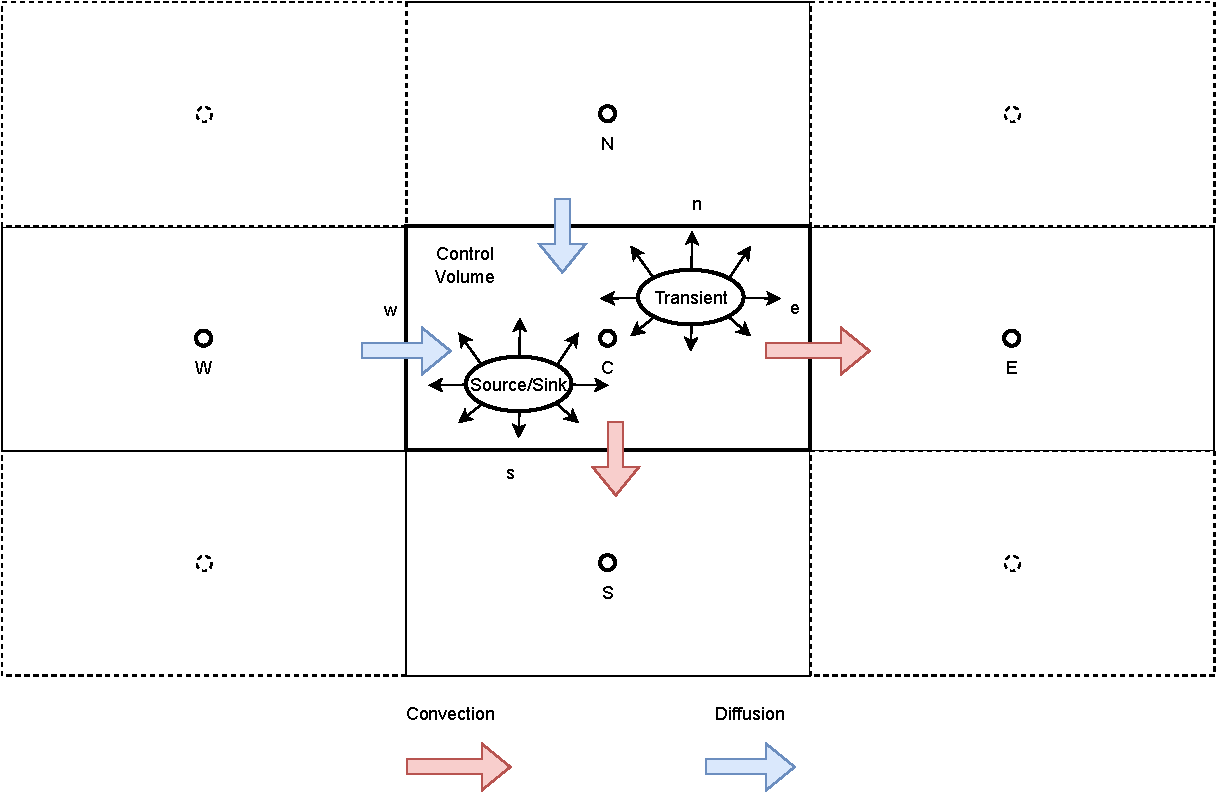
\includegraphics[scale=0.70]{Control_Volumen}
	\caption{Control Volume example}
	\label{fig:FVM_CV}
\end{figure}

From this point on it can be seen that the values of $\Phi$ at each cells surface are needed. The solution algorithm used calculates and stores the results only at the cells center. To obtain values at the cells surfaces the neighbouring cell's values are used as well. The method used here is called Quadratic upwind differencing scheme (QUICK) and is explained in greater detail within the following section.

\subsection{Quadratic upwind differencing scheme}
\label{sec:QUICK}

As shown in \autoref{fig:FVM_CV} each cell in a 2D case has 4 neighbouring cells that are labelled N for north, S for south, E for east and W for West. The approach used here is called \textbf{q}uadratic \textbf{u}pstream \textbf{i}nterpolation for \textbf{c}onvective \textbf{k}inetics \cite{versteeg2007introduction} or QUICK as an abbreviation. The QUICK method uses the 2 neighbouring cells upward the flow direction. A schematic is shown in \autoref{fig:QUICK}. The cell westward to the W cell is called WW and using the same naming scheme the cell eastward to E is named EE.
\begin{figure}[htbp]
	\centering
	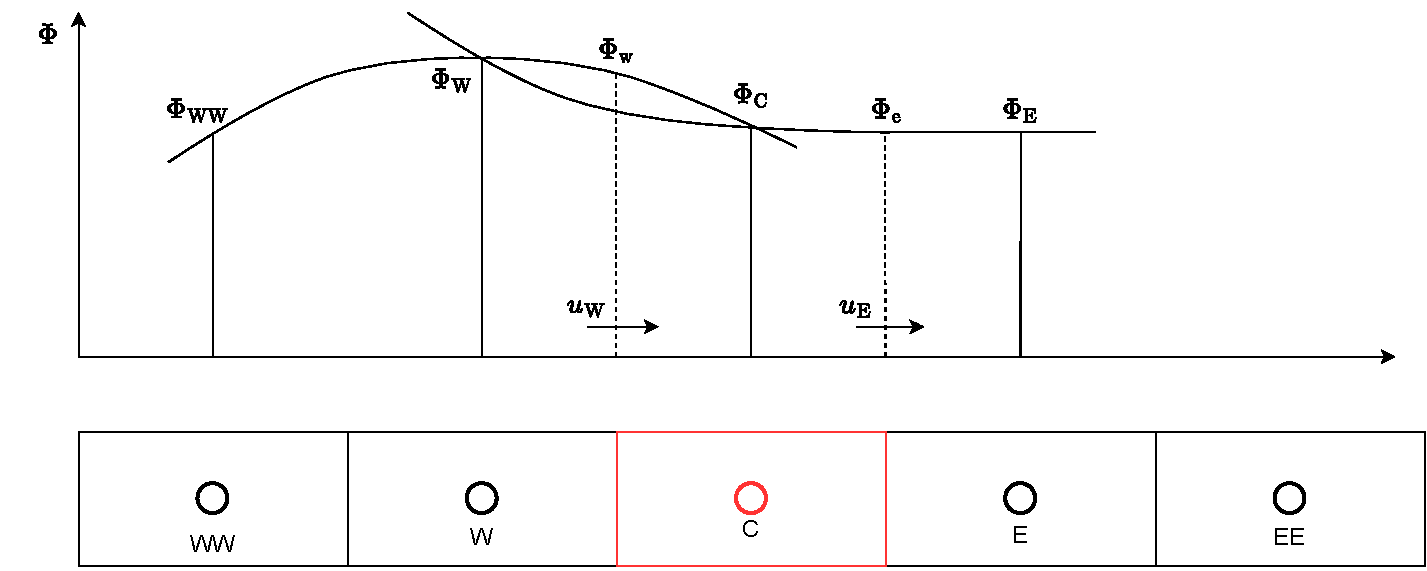
\includegraphics[scale=0.6]{QUICK}
	\caption{QUICK method cell scheme}
	\label{fig:QUICK}
\end{figure}
With a flow from west to east through the cell with the center C the cells surface values $\Phi_w$ for the west facing surface and $\Phi_e$ for the east facing surface are calculated as follows \cite{versteeg2007introduction}:
\begin{equation}
	\Phi_w = \dfrac{6}{8} \Phi_W + \dfrac{3}{8} \Phi_C - \dfrac{1}{8} \Phi_{WW}
\end{equation}
\begin{equation}
	\Phi_e = \dfrac{6}{8} \Phi_C + \dfrac{3}{8} \Phi_E - \dfrac{1}{8} \Phi_{W}
\end{equation}
It can be seen that the method highly values the cells value upstream given the weight value of $\frac{6}{8}$ since it has the most influence on the surface value it faces. If the flow is reverse in direction the method stays the same but the cells the values are used from do change.
\begin{equation}
	\Phi_w = \dfrac{6}{8} \Phi_C + \dfrac{3}{8} \Phi_W - \dfrac{1}{8} \Phi_{E}
\end{equation}
\begin{equation}
	\Phi_e = \dfrac{6}{8} \Phi_E + \dfrac{3}{8} \Phi_C - \dfrac{1}{8} \Phi_{EE}
\end{equation}

\section{Solution Method}
\label{sec:sol_method}

The solution method used in this case is called PISO algorithm which stands for \textbf{P}ressure \textbf{I}mplicit with \textbf{S}plitting \textbf{O}peration algorithm. A general overview of the method's procedure can be seen in \autoref{fig:PISO} \cite{versteeg2007introduction}.

\begin{figure}[htbp]
	\centering
	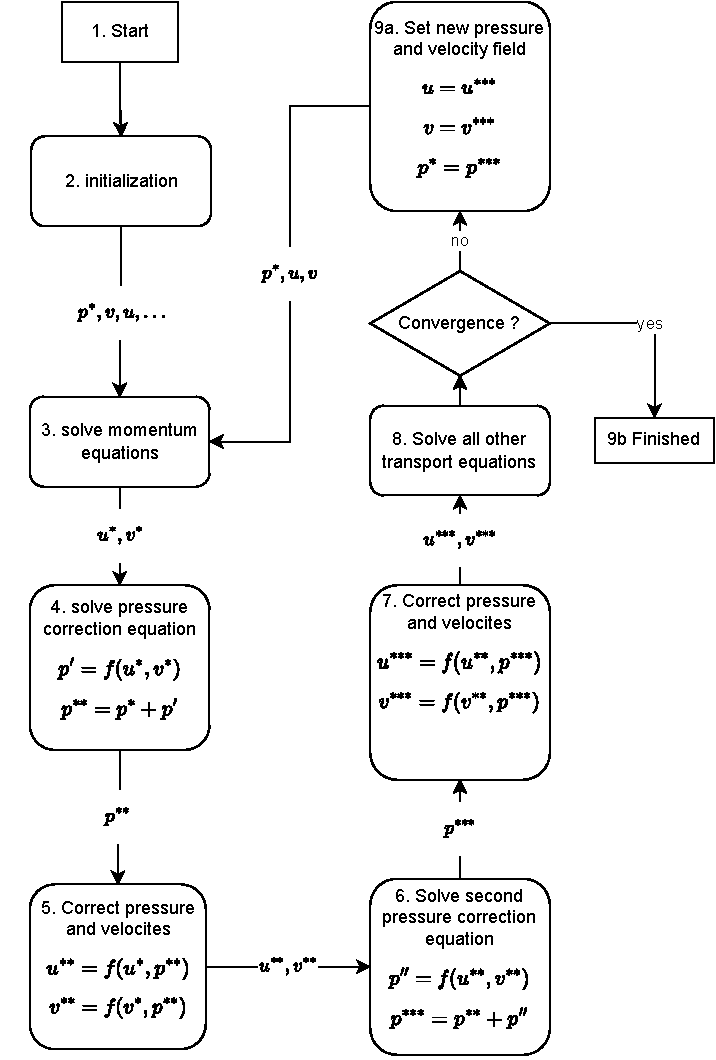
\includegraphics[scale=1.0]{PISO}
	\caption{PISO algorithm}
	\label{fig:PISO}
\end{figure}

At first all fields have to be initialized with some values given by the user. With these initial values the method starts its calculation. The first step within the calculation is to get the results of the momentum equations for each cell within the mesh. The results gained are, a 2D case given, the velocity fields $v^*$ and $u^*$. After this step is finished the gained velocity fields are used to calculate the pressure correction $p'$. This is done by setting the pressure offset to a value that satisfies the continuity equation for the cell. With this offset $p'$ a new pressure field $p^{**}$ can be calculated that is then used to correct the velocity fields $u^*$ and $v^*$. This correction is done in a way similar to the already described method in \autoref{sec:QUICK} using the values of the neighbouring cells. After the new velocity fields $u^{**}$ and $v^{**}$ have been gained the PISO algorithm performs a second pressure correction. This yields the pressure field $p^{***}$. Now a second velocity field correction takes place in the same manner as the first one. After that is done all other transport equations are solved using the latest fields for the velocities $u^{***}$, $v^{***}$ and the pressure $p^{***}$. Finally a convergence check is performed and if successful the algorithm stops. The convergence is a criterion that does a comparison of the fields that are given as inputs and the ones yielded as outputs. If their difference is bellow a certain set threshold the solution has converged. The threshold as to be given by the user for each variable of interest or the default ones are used. If the resulting fields have not converged the latest output is used as new input and the solving and corrections steps take place again. This iterative approach is done as long as the convergence criterion is not fulfilled or the maximum amount of iterations is reached.

\section{Flow Observations}

Within a developing reaction-diffusion-advection front some specific phenomena can be observed. The main ones are looked at in this section.

\subsection{Taylor-Dispersion}

The first phenomenon taking place within a reaction-diffusion-advection front is called Taylor-Dispersion. This was first discovered by G.I. Taylor\cite{aris1956dispersion} in 1956. The discovered phenomenon describes the spreading of a front over time as it can be seen within \autoref{fig: taylor_disp_pipe}. 
\begin{figure}[htbp]
	\centering
	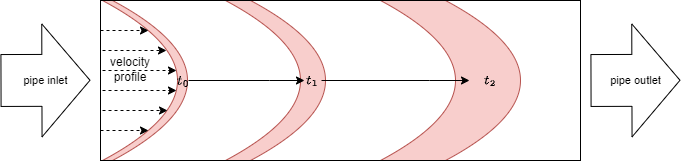
\includegraphics[scale=0.8]{taylor_dispersion_pipe}
	\caption{Taylor dispersion within a pipe reactor}
	\label{fig: taylor_disp_pipe}
\end{figure}
This simple example shows that the front, as marked in red within the image grows in width over time and distance. This growth process takes place due two diffusion within the front itself. Therefore the mixture's diffusion coefficient has a high influence on the fronts shape and how fast it grows. The hole effect is also affected by the inlets velocity magnitude. Within a tube such a poisseule flow develops if the velocity magnitude is below the critical one. This velocity can be calculated using the critical Reynolds number $Re_{crit}$ which in case of a tube has a value of $\approx 2300$. 
\begin{equation}
	\label{eqn: Re_crit}
	Re_{crit} = \dfrac{u_{crit} \cdot l}{\nu} \Leftrightarrow u_{crit} = Re_{crit} \cdot \dfrac{\nu}{l}
\end{equation}
With \autoref{eqn: Re_crit} the critical velocity can be calculated using the viscosity $\nu$ and the characteristic length $l$ which is in case of a tube the same as the tube's diameter $d$. With a velocity lower than the critical one a laminar velocity profile appears and the effect of Taylor dispersion can be visible.

Within the case of a radial reactor, that is investigated here, only gap averaged concentration values are available from the experiments. Within these experiments the effect of Taylor-Dispersion is visible within the data. A schematic \cite{levenspiel1998chemical} of this effect showing within the concentration data is displayed in \autoref{fig:taylor-disp}. The same effect can be observed within gas chromatography results for example which is a technique used in analytical chemistry.
\begin{figure}[htbp]
	\centering
	\includegraphics[scale=0.8]{taylor-dispersion}
	\caption{Taylor dispersion within a radial reactor \cite{levenspiel1998chemical}}
	\label{fig:taylor-disp}
\end{figure}

As shown in \autoref{fig:taylor-disp} the fronts concentration distribution changes along the flow direction $x$ within the time $t$. The peak lowers and the distribution widens as time passes. How quickly this effect takes place and which parameters have a significant influence is discussed within \autoref{chp: para_stud}. Within this work the front's width as well as the height averaged concentration distribution are the results looked at when checking this phenomenon.

\subsection{Reaction Details}
\label{sec: reaction_details}

Within this section a closer look is taken at the reaction that is implemented in the model. The reaction can be described by \autoref{eqn: reaction_detail}.

\begin{equation}
	\label{eqn: reaction_detail}
	A + B \xrightarrow{r} C
\end{equation}

The reaction rate $r$ can be calculated using \autoref{eqn: reaction_vel}. From this equation it can be seen that the reaction is of second order and is dependent of the species $A$ and $B$.

\begin{equation}
	\label{eqn: reaction_vel}
	r = k \cdot c_A \cdot c_B
\end{equation}

The reaction velocity equation uses the rate constant $k$ which can be computed using the context of \autoref{eqn: reaction_rate_detail}.

\begin{equation}
	\label{eqn: reaction_rate_detail}
	k = k_{\infty} \cdot e^{- \frac{E_A}{R \cdot T}}
\end{equation}

Since the reaction needs to be nearly instantaneous as mentioned in \autoref{sec: reaction_eqn} the pre-exponential factor $k_{\infty}$ is set to a high value of $10^{15} \left[ \frac{\text{l}^2}{\text{mol} \cdot \text{s}} \right] $. The reaction takes place under isothermal conditions so the rate has a constant value. The variable $E_A$ is the reaction's activation energy with a value of $10^4 \left[ \frac{\text{J}}{\text{mol}} \right] $, $R$ is the gas constant with a value of 8.3145 $\left[ \frac{\text{J}}{\text{mol} \cdot \text{K}} \right] $ and $T$ is the temperature in Kelvin. The activation energy only needs to fulfill the requirement that the reaction takes place under the given temperature conditions.

\subsection{Dimensionless Variables}

To be able to compare simulations and experiments two dimensionless variables are used. These are the Schmidt number $Sc$ and the Peclet-Number $Pe$. The Peclet-Number is calculated using \autoref{eqn: Pe} and the Schmidt number is computed using \autoref{eqn: Sc}.

\begin{equation}
	\label{eqn: Pe}
	Pe = \dfrac{l \cdot u}{D}
\end{equation}

The Peclet-Number is influenced by the characteristic length $l$ as known from the Reynolds number, the input velocity $u$ and the diffusion coefficient $D$. The characteristic length within this model is equal to the gap height. The diffusion coefficient is set to be the same one as calculated from the experiments for model validation but is also varied when doing the parametric study.

\begin{equation}
	\label{eqn: Sc}
	Sc = \dfrac{\nu}{D}
\end{equation}

The Schmidt number is only influenced by species constants. The already mentioned diffusion constant $D$ and the viscosity $\nu$ affect this variable. Both are adapted when changing $Sc$ during the parametric study.

In addition to the Schmidt-Number and the Peclet-Number the Courant-Number plays a role in the development process. This number is only used for mesh grid size determination. This number can be calculated using \autoref{eqn:cfl}. It is influenced by the velocity $u$, the time step $ \Delta t$ and the spacial discretization $\Delta x$.

\begin{equation}
	\label{eqn:cfl}
	c = \dfrac{u \cdot \Delta t}{\Delta x}
\end{equation}

\end{document}